\documentclass[12pt]{article}
\usepackage[utf8]{inputenc}
\usepackage[T2A]{fontenc}
\usepackage[mongolian]{babel}
\usepackage{graphicx}


\title{Их дээд сургуулийн мэдээллийн веб}

\begin{document}
	\maketitle
		\section{Системийн шаардлага}
		\begin{itemize}
			\item Систем нь веб суурьтай байх.
			\item Системийг ашиглахын тулд заавал сүлжээнд холбогдсон байх.
			\item Google хаягаар бүртгүүлэх боломжтой байх.
			\item Гаргасан хийх зүйлсийн жагсаалтуудыг хэвлэх боломжтой байх.
		 	
		\end{itemize}
	\section{Системийн хэрэглэгчид}
	\begin{itemize}
		\item Багш
		\item Оюутан
		\item Хичээл зохицуулагч
	\end{itemize}
\section{Функционал шаардлага}
\begin{enumerate}
	\item Багш
	\begin{enumerate}
		\item Багш өөрийн орох цагуудаа харах
		\item Багш өдрөөр, хичээлээр ангилан харах
	\end{enumerate}
	\item Оюутан
	\begin{enumerate}
		\item Оюутан хуваарь харах
		\item Оюутан хуваариа баталгаажуулах хүсэлт илгээх
		\item Оюутан хичээлийн хуваариа хэвлэх
	\end{enumerate}
	\item Хичээл зохицуулагч
	\begin{enumerate}
		\item Хичээлийн хуваарь гаргах
		\item Оюутны хүсэлтийг баталгаажуулах
		\item Цаг нэмэх 
		\item Цаг хасах
	\end{enumerate}
\section{Функциональ бус шаардлага}	
\begin{itemize}
	\item Хуудас хооронд хурдан шилжих
	\item Хүн удаан харахад нүд ядрахгүй байх
	\item Системийн загвар хүнд ойлгомжтой байх	
\end{itemize}
\end{enumerate}
\begin{figure}
	\centering
	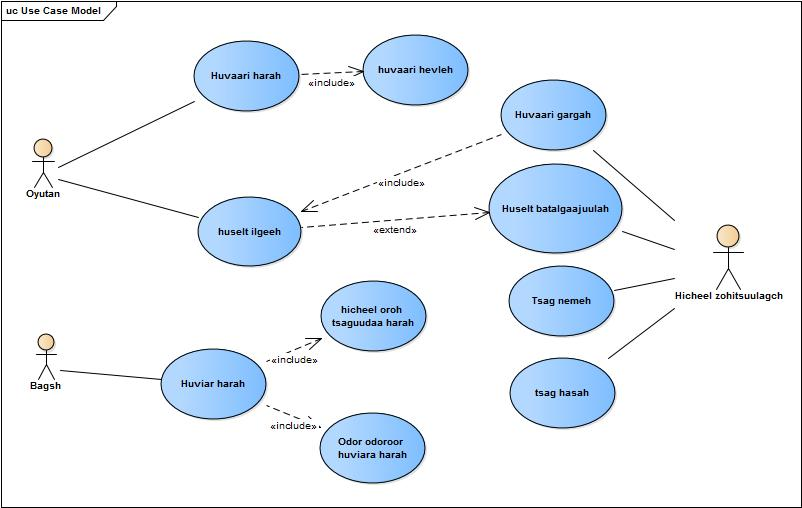
\includegraphics[width=1\textwidth]{diagrams/use-case}
	\caption{Use-Case диаграм}
	\label{fig:use-case-model}
\end{figure}
	
\end{document}